\scanpage{32}
\margin{31}
% Une longue barre oblique traverse le corps du feuillet.
\deleted{
\uline{Case} a) The construction \inserted{\unsure{is not}} \unsure{able to} continue \unsure{indefinitely}
i.e. we end up having $\sigma a_n\notin A'$, we then \unsure{set}
$\sigma a_n=\rho a_0$.

\uline{Case} b) The construction continues \unsure{indefinitely}.

(\deleted{\unsure{whether} \unsure{we} \inserted{\unsure{therefore}} \unsure{have a finite cycle}}, \unsure{or an}
\unsure{infinite} cycle). We do not \unsure{define} $\rho\unsure{\widehat a|a}$ \unsure{then}.

\margin{\figure{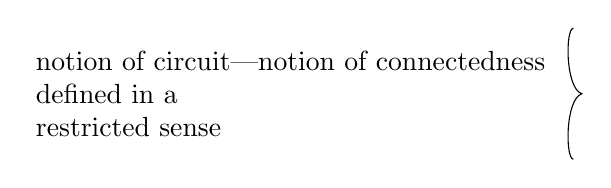
\begin{tikzpicture}
\node[align=left,inner sep=3pt] (m) {\unsure{notion of circuit|notion of connectedness}\\\unsure{defined in a}\\\unsure{restricted sense}};
\draw ([xshift=7pt,yshift=5pt]m.north east)
 .. controls ([xshift=4pt,yshift=5pt]m.north east) and ([xshift=4pt,yshift=2pt]m.east) .. ([xshift=10pt]m.east)
 .. controls ([xshift=4pt,yshift=-2pt]m.east) and ([xshift=4pt,yshift=-5pt]m.south east) .. ([xshift=7pt,yshift=-5pt]m.south east);
\end{tikzpicture}}}
We suppose henceforth that $\rho$ is \deleted{\unsure{defined}} \inserted{\unsure{extended}} on \unsure{all of} $A$
and that \unsure{$=$} for the \unsure{opposite} orientation (these are
\unsure{combinatorial} properties of $(A,\sigma,A',\rho)$).
Then $\rho$ on $A$ is an \uline{\unsure{automorphism}}. Let $\unsure{\overline S}=A/\rho\supset S$,
$\widehat S\unsure{\subset|=}\overline S$ the subset of $\overline S$ corresponding to the finite orbits.
We can \unsure{compactify} \unsure{partially} $X$ to \inserted{$\widehat X$}\deleted{\unsure{$\overline X$}}
\unsure{adding} the points of $\widehat S-S$ (as well
as : $\unsure{K^\circ}$\inserted{\unsure{$\simeq\Pi_{0,3}$}}), the inverse image \inserted{$\widehat A'$} of
$\widehat S$ in $A$ \inserted{\unsure{contains $A'$ and}}
is \unsure{stable} \unsure{$\forall$} under $\rho$ and $\sigma$
but \deleted{\unsure{is not|this is not} necessarily equal \unsure{to|with} $A'$.}
\inserted{: $A$ \unsure{in its entirety|is entire}.}

\margin{\figure{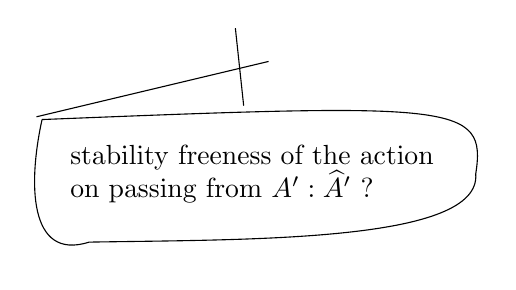
\begin{tikzpicture}
\node[align=left,inner sep=5pt] (m) {\unsure{stability freeness of the action}\\\unsure{on passing from} $A':\widehat A'$ ?};
\draw ([xshift=-5pt,yshift=4pt]m.north west)
 .. controls ([xshift=-10pt,yshift=-3pt]m.west) and ([xshift=-10pt,yshift=-16pt]m.south west) .. ([xshift=12pt,yshift=-9pt]m.south west)
 .. controls ([yshift=-8pt]m.south) and ([xshift=12pt,yshift=-9pt]m.south east) .. ([xshift=10pt]m.east)
 .. controls ([xshift=14pt,yshift=10pt]m.north east) and ([xshift=3pt,yshift=10pt]m.north east) .. ([xshift=-5pt,yshift=4pt]m.north west);
\draw ([xshift=-7pt,yshift=5pt]m.north west) -- ([xshift=6pt,yshift=25pt]m.north);
\draw ([xshift=-3pt,yshift=9pt]m.north) -- ([xshift=-6pt,yshift=37pt]m.north);
\end{tikzpicture}}}

The quadruples $(A,\sigma,A',\rho)$ \unsure{satisfying} the
axioms, \unsure{must} \inserted{and such that $A'=\widehat A'$}
\unsure{be identified|are identified} with the \deleted{\unsure{triples}} triples
$(A,\sigma,\rho)$ of a set \uline{\unsure{whatsoever}} with an automorphism
$\sigma$ of order $2$ \uline{without a fixed point}, and an automorphism $\rho$
\uline{whatsoever}. We \unsure{recover} $A'$ as the set of
elements of $A$ with finite orbit under $\rho$ --- but we
suppose that $A'\cup\sigma A'=A$.
}

\scanpage{33}
\diagram{\begin{tikzcd}[ampersand replacement=\&,column sep=large,row sep=large]
 0\arrow[r] \& \overset{\omega}{\mathbb Z}\arrow[r,"p"]\arrow[d,"q"'] \& \overset{\widetilde\Pi_0}{\overset{\Vert}{\mathbb Z}}\arrow[r,"\alpha\varphi_p",very thick]\arrow[d] \& \overset{\Pi_0}{\overset{\Vert}{\mathbb Z/p\mathbb Z}}\arrow[r]\arrow[d,equal] \& 0\\
 0\arrow[r,no head,"\overline\omega"'] \& \mathbb Z\arrow[r] \& \widetilde\Pi_0(q)\arrow[r]\arrow[d,"{\substack{\text{\unsure{zero on }}\widetilde\Pi_0,\\\text{\unsure{canonical on }}\mathbb Z\overline\omega}}"] \& \mathbb Z/p\mathbb Z\arrow[r,no head] \& 0\\
 \&\& \mathbb Z/q\mathbb Z \&\&
\end{tikzcd}}
\margin{$\varphi_p:\mathbb Z\longrightarrow\mathbb Z/p\mathbb Z$ canonical homomorphism\\
$\alpha\in(\mathbb Z/p\mathbb Z)^*$\\
\deleted{$\unsure{\beta}\in(\mathbb Z/q\mathbb Z)^*$}}

\diagram{\begin{tikzcd}[ampersand replacement=\&,column sep=large,row sep=large]
 \&\& \overset{\omega}{\mathbb Z}\arrow[r]\arrow[dl,equal] \& \widetilde\Pi_0\arrow[r]\arrow[dl] \& (\mathbb Z/p\mathbb Z\times0)\arrow[dl]\\
 0\arrow[r,no head] \& \overset{\omega}{\mathbb Z}\arrow[r]\arrow[dr,shift right=.6ex] \& \widetilde\Pi_0(q)\arrow[r] \& \mathbb Z/p\mathbb Z\times\mathbb Z/q\mathbb Z\arrow[r,no head] \& 0\\
 \&\& \underset{\omega}{\mathbb Z}\arrow[ul,"q"'{pos=.55},shift right=.6ex]\arrow[r,"\unsure{q}"] \& \underset{\overline\omega}{\mathbb Z}\arrow[ul]\arrow[r,no head] \& 0\times\mathbb Z/q\mathbb Z\arrow[ul]
\end{tikzcd}}
\margin{$\alpha\eta_p$}

\diagram{\begin{tikzcd}[ampersand replacement=\&,column sep=large,row sep=large]
 0\arrow[r,no head] \& \mathbb Z\arrow[r]\arrow[d,equal] \& \widetilde\Pi_0(q)\arrow[r,no head] \& \mathbb Z/p\mathbb Z\times\mathbb Z/q\mathbb Z\arrow[r,no head] \& 0\\
 0\arrow[r,no head] \& \mathbb Z\arrow[r,no head] \& \widetilde\Pi'_0\arrow[r]\arrow[u] \& \mathbb Z/\mu\mathbb Z\arrow[r,no head]\arrow[u,"\delta",very thick] \& 0
\end{tikzcd}}

\deleted{\unsure{The extension is} \illegible{1} :}
\[
 \unsure{\zeta'|\xi'}\deleted{\unsure{\zeta|\xi}}=
 \mathrm{cl}(\widetilde\Pi'_0)\in
 \operatorname{Ext}^{\unsure{1}}_{\deleted{\unsure{\mathbb Z}}}
 (\mathbb Z/\mu\mathbb Z,\mathbb Z)\simeq\mathbb Z/\mu\mathbb Z
\]
\[
 \deleted{\unsure{=}}\quad
 \unsure{\zeta'|\xi'}=
 \delta^*\!\left(
 \underbrace{\mathrm{cl}(\widetilde\Pi_0\unsure{(q)|q})}_{\unsure{\zeta|\xi}\,\in\,\operatorname{Ext}^1(\mathbb Z/p\mathbb Z\times\mathbb Z/q\mathbb Z,\mathbb Z)}
 \right)\unsure{'}
\]
\[
 \unsure{\zeta|\xi}=
 \mathrm{pr}_1^*\!\left(\underbrace{\mathrm{cl}(\widetilde\Pi_0)}_{\alpha\eta_p}\right)
 +\mathrm{pr}_2^*\!\left(\underbrace{\mathrm{cl}(\mathbb Z)}_{\eta_q}\right)
\]
\[
\begin{array}{ll}
 \delta_p:\mathbb Z/\mu\mathbb Z\mathrel{\overset{\mathrm{can}}{-}}\mathbb Z/p\mathbb Z
 &\unsure{\zeta'|\xi'}=\deleted{q'\eta_\mu+p'\eta_\mu}\\[1ex]
 \delta_q:\mathbb Z/\mu\mathbb Z\mathrel{\overset{\mathrm{can}}{-}}\mathbb Z/q\mathbb Z&\\[1ex]
 \delta_p^*(\eta_p)=q'\eta_\mu & \delta_p^{\unsure{*|' }}(\alpha\eta_p)=q'\alpha\eta_\mu\\[1ex]
 \delta_q^{\unsure{*|'}}(\eta_q)=p'\eta_\mu &
\end{array}
\]
\margin{32}

\scanpage{34}
\deleted{$\unsure{4)}\ \unsure{\widetilde{\mathrm{Sl}}}(2,\mathbb Z)\simeq
\unsure{\mathcal T_{1,1}}\,\unsure{\mathrm{SL}}\,\unsure{\Pi}$}

1)
\[
\begin{gathered}
 S\mathcal T_{11}\simeq\widetilde{\mathrm{Sl}}(2,\mathbb Z)
 \simeq\{\rho,\sigma\mid\underbrace{\rho^3=\sigma^2}_{\omega}\}
 \simeq
 \underset{\substack{\Vert\\\{\rho,\sigma\mid\rho^3=\sigma^2=1\}}}{\Pi_{0,3}^D}
 \times_{\unsure{\mathbb Z/6\mathbb Z}}\mathbb Z\\
 \simeq S\Pi_{0,3}^D
\end{gathered}
\]
\inserted{\deleted{$\unsure{\alpha}$}
\diagram{\begin{tikzcd}[ampersand replacement=\&,row sep=small]
 \rho\arrow[r,mapsto]\&2\\
 \sigma\arrow[r]\&3
\end{tikzcd}}}

% Le bloc suivant est écrit tête-bêche par rapport à la ligne précédente.
\diagram{\begin{tikzcd}[ampersand replacement=\&,column sep=large,row sep=large]
 \widetilde\Pi\arrow[r,no head]\arrow[dd,no head]\&\unsure{\Pi}\arrow[r,no head]\arrow[d]\&\Pi'\arrow[r]\arrow[dd,Rightarrow]\&\Pi\arrow[dd]\\
 \&\mathbb D_3''\arrow[dd]\&\&\\
 \mathbb Z\arrow[rr]\&\&\mathbb Z/12\mathbb Z\arrow[r]\arrow[d]\&\mathbb Z/6\mathbb Z\arrow[d]\\
 \&\unsure{\mathbb Z/}\&\mathbb Z/4\mathbb Z\arrow[r]\&\mathbb Z/2\mathbb Z
\end{tikzcd}}
\margin{$\Pi_0=\mathbb Z/6\mathbb Z$}
\margin{$\Pi_0\times\unsure{7|1}$}
\diagram{\begin{tikzcd}[ampersand replacement=\&,column sep=large,row sep=large]
 \mathbb Z\arrow[r,no head]\&\widetilde\Pi(4)\arrow[r]\&\Pi\times\mathbb Z/4\mathbb Z\arrow[r,no head]\arrow[d]\&1\\
 \&\widetilde\Pi\arrow[u,"?"']\arrow[r,"\uline{\unsure{cart}}"]\&\Pi'\&
\end{tikzcd}}

% Billet préexistant, à lire après une rotation de 90 degrés.
\margin{27-11-81}
Mr. Grothendieck

To be filled out urgently

Thank you

\uline{R. \unsure{Boucher}}
\margin{33}

\scanpage{35}
\[
 (p'+q'\alpha)\eta_\mu
\]
\[
 p=6,\ q=4\qquad(\alpha=-1\ ?)
\]
\[
 \deleted{\unsure{p}}\ \mu=12\qquad p'=3,\ q'=2
\]
\[
 \deleted{\unsure{p'+}}\ (3-2)\eta_\mu\ !
\]
\figure{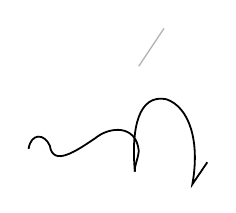
\begin{tikzpicture}[x=1cm,y=1cm]
 \draw[line width=.5pt,opacity=.3] (1.4,1.7)--(1.72,2.18);
 \draw[line width=.65pt] (0,.65) .. controls (.03,.85) and (.2,.85) .. (.27,.69)
 .. controls (.31,.42) and (.6,.62) .. (.84,.78)
 .. controls (1.03,.94) and (1.37,.96) .. (1.4,.62)
 .. controls (1.38,.48) and (1.34,.43) .. (1.35,.36);
 \draw[line width=.65pt] (1.35,.36) .. controls (1.3,.92) and (1.4,1.35) .. (1.75,1.28)
 .. controls (2.04,1.18) and (2.18,.75) .. (2.08,.2)
 --(2.27,.48);
\end{tikzpicture}}

$\cdot$
\diagram{\begin{tikzcd}[ampersand replacement=\&,column sep=large,row sep=small]
 \Pi_{0,3}^D\arrow[r,"{-\alpha}"{draw,circle,inner sep=1pt},very thick]\&\mathbb Z/6\mathbb Z\\
 \rho\arrow[r,mapsto]\&-2\ \mathrm{mod}\ 6\\
 \sigma\arrow[r,mapsto]\&3\ \mathrm{mod}\ 6\\[1ex]
 \varepsilon_0=\sigma\rho\arrow[r,mapsto,very thick]\&1\ \mathrm{mod}\ 6\\
 \rho_0=\varepsilon_0^2\arrow[r,mapsto]\&2\ \mathrm{mod}\ 6
\end{tikzcd}}
\deleted{$\unsure{\varphi}$}
% Marques très pâles à droite des résidus; possible transparence du verso.
\margin{$\unsure{\Gamma|\sqrt{\phantom{x}}}$\\$\unsure{\xi_0\prime|\xi_0}$\\$\unsure{t\prime r|t\prime h}$}

\margin{defined directly by the action of $\Pi_{0,3}^D$ on the
principal \unsure{cover}\deleted{\unsure{ing}} of $(U_{0,3},\mathfrak S_3)$
with group $\mathbb Z/6\mathbb Z$, defined by
the \inserted{canonical} \unsure{multisection|multiplication} of
\deleted{$\unsure{\mathcal O(1)}$}$\mathcal O_{U_{0,3}}(1)^*$
$=PU_{0,3}$}

\[
 \widetilde\Pi_{0,3}^D
\]
\deleted{$\mathcal O\unsure{(1)}$}
\diagram{\begin{tikzcd}[ampersand replacement=\&,column sep=small,row sep=large]
 U'_{0,3}\arrow[rr,phantom,"\subset"]\arrow[dr,no head,"{\mu_6\text{-}\unsure{\mathrm{rev}^{\mathrm t}}}"']\&\&PU_{0,3}\arrow[dl,no head]\&\unsure{+}\\
 \&U_{0,3}\&\&
\end{tikzcd}}
\deleted{$\unsure{\longrightarrow}$}

\diagram{\begin{tikzcd}[ampersand replacement=\&,column sep=large,row sep=large]
 \&\Pi_{0,3}^D\arrow[r,"{\alpha'}"{draw,circle,inner sep=1pt},very thick]\&\mathbb Z/6\mathbb Z\\
 \pi_1(PU_{0,3},\mathfrak S_3)\arrow[r,equal]\&\widetilde\Pi_{0,3}^D\arrow[u]\arrow[r]\&\mathbb Z\arrow[u]\\
 \&\omega'\in\mathbb Z\arrow[u]\arrow[r,"\unsure{=}"]\&\mathbb Z\arrow[u,"6"]
\end{tikzcd}}

\diagram{\begin{tikzcd}[ampersand replacement=\&,column sep=large,row sep=large]
 1\arrow[r]\&\mathbb Z\arrow[r]\arrow[d,equal]\&
 \underset{\substack{\Vert\\\pi_1(PU_{0,3},\mathfrak S_3\times\mu_4)}}{\widetilde\Pi_{0,3}^D(4)}\arrow[r,very thick]\&
 \Pi_{0,3}^D\times\mathbb Z/4\mathbb Z\arrow[r]\&1\\
 1\arrow[r,no head]\&\mathbb Z\arrow[r]\&\widetilde{\mathcal T}_{11}\arrow[u,bend left=20]\arrow[r,Rightarrow]\&
 \mathcal T_{1,1}=\Pi_{0,3}^D\times_{\mathbb Z/2\mathbb Z}\mathbb Z/4\mathbb Z\arrow[u,hook]\&
\end{tikzcd}}

\deleted{$\unsure{\widetilde\Pi_{0,3}^D}\,\unsure{\mathbb Z/4\mathbb Z}\longrightarrow$}
\[
\begin{array}{ll}
 \widetilde\Pi_{0,3}^D\ni\widetilde\rho^{\unsure{\sharp|'}}=(\rho,-2)
 &\widetilde\rho^{\unsure{\sharp}3}=\widetilde\sigma^{\unsure{\sharp}2}=\omega'\\
 \hfill\widetilde\sigma^{\unsure{\sharp|'}}=(\sigma,-3)&
\end{array}
\]
\diagram{\begin{tikzcd}[ampersand replacement=\&,column sep=small,row sep=small]
 \widetilde\rho,\arrow[d]\&\widetilde\sigma\arrow[d]\&
 \in\widetilde\Pi_{0,3}^D=
 \left\{\widetilde\rho,\widetilde\sigma\mid
 \underbrace{\widetilde\rho^3=\widetilde\sigma^2}_{\unsure{\omega'^{-1}|\widetilde\omega^{-1}}=\unsure{\omega|\infty}}
 \deleted{\unsure{\omega\in\mathbb Z}}\right\}\\
 \rho\&\sigma\&\simeq\widetilde{\mathcal T}_{11}
\end{tikzcd}}
\margin{34}

\scanpage{36}
\diagram{\begin{tikzcd}[ampersand replacement=\&,column sep=large,row sep=large]
 \&\&\left\{\rho,\sigma\mid\underbrace{\rho^3=\sigma^2}_{\omega'^{-1}=\omega}\right\}\deleted{\unsure{\omega|\infty}}\arrow[d,equal]\&\&\\
 1\arrow[r,no head]\&\overset{\omega'=\unsure{\omega^{-1}|\overline\omega'}}{\mathbb Z}\arrow[r]\arrow[d,equal]\&S\Pi_{0,3}^D\arrow[r]\arrow[d]\&\Pi_{0,3}^D\arrow[r,no head]\arrow[d]\&1\\
 1\arrow[r,no head]\&\mathbb Z\arrow[r]\&S\Pi_{0,3}^D(4)\arrow[r]\&\Pi_{0,3}^D\times\mathbb Z/4\mathbb Z\arrow[r,no head]\&1\\[4em]
 1\arrow[r]\&\underset{\omega^2}{\mathbb Z}\arrow[r]\arrow[u,very thick]\&S\mathcal T_{11}\arrow[r]\arrow[u,very thick,"{\underbrace{\begin{gathered}\rho\mapsto\rho\overline\omega^2\\\sigma\mapsto\sigma\overline\omega^3\\\omega\longrightarrow\overline\omega^2\\\omega^2\longrightarrow\overline\omega^4=\omega'\end{gathered}}}"]\&\mathcal T_{11}\arrow[u,hook,"{\substack{\rho\mapsto(\rho,2)\\\sigma\mapsto(\sigma,3)}}"]\&\omega\longrightarrow(1,2)
\end{tikzcd}}
\margin{$S\Pi_{0,3}^D(4)=\left\{\rho,\sigma,\overline\omega\mid\begin{gathered}\rho^3=\sigma^2=\overline\omega^{-4}\\\overline\omega\ \text{central}\end{gathered}\right\}$\\
N.B. $\unsure{\dot{\overline\omega}|\overline\omega}^{4}=\unsure{\omega^{-1}}$\\
$=\omega'\deleted{\unsure{\omega}}$}

% Groupe et flèche au pied du feuillet, écrits tête-bêche.
\diagram{\begin{tikzcd}[ampersand replacement=\&,column sep=large]
 \overbrace{S\Pi_{0,3}^D(4)}^{\pi_1(U_{0,3},\mathfrak S_3\times\mu_4)}\arrow[r]\&\Pi_{0,3}^D
\end{tikzcd}}
\margin{35}

\scanpage{37}
% not manuscript: formulaire vierge « ANNEXE II », renseignements à fournir par le candidat devant soutenir une thèse de doctorat d'État, Université des Sciences et Techniques du Languedoc, imprimé tête-bêche.
\margin{36}